\documentclass[11pt,letterpaper]{article}

\usepackage[letterpaper,margin=0.8in,nohead]{geometry}

\usepackage[colorlinks]{hyperref}
\usepackage{url}
\usepackage{breakurl}

\hypersetup{
	colorlinks,
	linkcolor={red},
	citecolor={red},
	urlcolor={blue}
}

\usepackage{verbatim}
\usepackage{fancyvrb}
\usepackage{scrextend}
\usepackage{enumitem}
\usepackage{url}
\usepackage{subcaption}

\usepackage{filecontents}
%\usepackage{natbib}
%\nobibliography*

\usepackage{caption}
\usepackage{graphicx}

\usepackage{changepage}   % for the adjustwidth environment

\newenvironment{answer}{\em \color{blue} \begin{adjustwidth}{1cm}{1cm}}{\end{adjustwidth}}

% math
\usepackage{amsthm,amsmath}
\usepackage{amsfonts}

\newcommand{\mc}[1]{\mathcal{#1}}	% Mechanisms / Algorithms
\newcommand{\rv}[1]{\mathbf{#1}}    % Random variable

\newcommand{\pr}[1]{\mathrm{Pr}\{#1\}} % Probability

\newtheorem{corollary}{\bf Corollary}%[theorem]
\newtheorem{lemma}{\bf Lemma}%[theorem]
\newtheorem{definition}{\bf Definition}%[section]

\newtheorem{observation}{\bf Observation}%[theorem]



% load cleveref last!
\usepackage[capitalise]{cleveref}

\crefname{observation}{Observation}{Observations}


\begin{document}
	
	\title{EN4720: Security in Cyber-Physical Systems \\ Programming Assignment --- Passwords}
	
	%% This is an individual assignment!!
	%% TODO: put your name and index number here here!
	\author{ \textcolor{blue}{Name: Thalagala B. P.} \\ \textcolor{blue}{Index No: 180631J}}
	
	\maketitle
	
	\begin{center}
		\color{red}\bf This is an individual assignment! \\ Due Date: 8 July 2023 by 11.59 PM
	\end{center}
	
	\begin{center}
		\small Content adopted from {\bf CNT5410 Computer and Network Security} taught by Prof. Vincent Bindschaedler at the University of Florida.
	\end{center}
	
	\section*{Instructions}
	%
	
	Please read the instructions and questions carefully. Write your answers directly in the space provided. Compile the tex document and hand in the resulting PDF as your report.
	
	In this assignment, you will write a few lines Python code. You are encouraged to use Python3. You will need the PyCrypto library to run the provided code. Please refer to resources specific to your operating system and environment for installation instructions\footnote{\url{https://pypi.org/project/pycrypto/} See also:  \url{https://www.pycryptodome.org/en/latest/index.html}.}. For example, you can use: \texttt{pip3 install pycrypto} to install PyCrypto with Python3 under Linux.
	
	\subsection*{Assignment Files}
	The assignment archive contains the following Python source files:
	%
	\begin{itemize}[nolistsep]
		\item \texttt{utils.py}. This file contains utility functions needed for the assignment..
		\item \texttt{crypto.py}. This file defines cryptographic functions. 
		\item \texttt{attack.py}. This file contains attack code used in the assignment.
	\end{itemize}
	
	\noindent
	In addition, the assignment archive contains a \texttt{data} directory which includes a dictionary file (\texttt{words.list}) and several database dump files in JSON format (\texttt{*-dbdump.json}).
	
	\subsection*{Submission}
	Write your answers directly in the space provided. Compile the tex document and submit the resulting PDF together with the source code in a single zip file through Moodle.
	
	\bigskip
	
	\noindent
	\underline{Note:} \\
	\noindent You are encouraged to take a look at the provided files. This may help you successfully complete the assignment. \\
	\noindent 
	You might have to change the line ``from Cryptodome.Hash import SHA256'' in crypto.py to ``from Crypto.Hash import SHA256'' based on your OS and library versions. \\
	\noindent
	The program can take a while to run and the terminal might not show anything until program execution is complete. But it should not take more than 5 minutes (max).
	
	\newpage
	\section*{Problem 0: Bruteforce attack (12 pts)}
	%
	In this problem, you will mount a bruteforce attack against a stolen database dump of password hashes (\texttt{data/simple-dbdump.json}). The code for this problem is already written. (But you are encouraged to take a look to see how it works.)
	
	The bruteforce attack will try all possible passwords of 4 (or less) alphanumeric characters --- lowercase only. To perform the attack run the following command\footnote{You may have to specify to use Python3 \texttt{python3} if you also have Python2 versions installed on your system.}:
	%
	\begin{Verbatim}
		python attack.py problem0
	\end{Verbatim}
	%
	
	\begin{enumerate}
		
		\item (2 pts) What steps can you take to create a password that is hard to crack using bruteforce attacks?
		
		\begin{answer}
			
			\begin{itemize}
				\item A \textbf{combination of numbers, letters (upper case and/or lower case)  and special characters} must be used. This make the number of options per character to be large which eventually make it hard to brute-force.
				
				\item \textbf{The password must be sufficiently long}. This makes the number of possible password combinations (password space) extremely large which will make the brute-force attack computationally infeasible to be done in a shorter period of time. 
			\end{itemize}
			
		\end{answer}
		
		\item (4 pts) Which passwords are recovered (for which users)? How long did the attack take (in seconds)? What was the speed of the attack (in hashes/second)? Add a screenshot of your terminal output showing the answer.
				
		
		\begin{answer}
			
			\begin{figure}[h]
				\centering
				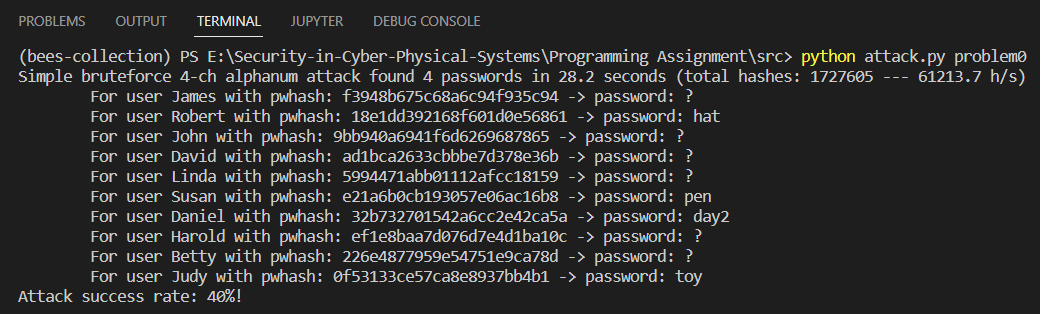
\includegraphics[width=0.8\columnwidth]{images/p0/q1.png}
				\caption{Output of the {\tt python attack.py problem0}}
			\end{figure}
			
			\begin{itemize}
				\item Time for the attack = 28.2 seconds
				\item Speed of the attack = 61213.7 hashes per second
				\item Attack success rate: 40\%				
			\end{itemize}
			
			\begin{table}[h]
				\centering
				\begin{tabular}{|l|l|}
					\hline
					\textbf{User} & \textbf{Password} \\ \hline
					Robert & hat \\ \hline
					Susan & pen \\ \hline
					Daniel & day2 \\ \hline
					Judy & toy \\ \hline
				\end{tabular}
				\caption{Recovered Passwords}
			\end{table}			
			
		\end{answer}
		\pagebreak
		\item (2 pts) What is the total number of {\em possible} passwords of $l$ {\em or less} alphanumeric characters --- lowercase only? 
		
		\begin{answer}
			
			Since there are 26 lowercase letters and 10 digits, there are a total of 36 possible characters that can be used in each position of the password. For a password of length $n$, there are $36^n$ passwords. If we consider the passwords of length l and less, we can have the following number of total passwords, which is the sum of a geometric series where number of terms equal to $l$, common ratio is 36 and the first term is 36.
			
			\begin{equation}
				\sum_{n=1}^{l} 36^n = 36 \cdot \frac{36^l -1}{36 - 1} = \frac{36^{l+1}-36}{35}
			\end{equation}
			
			In addition, the program considers an empty string ({\tt `'})  as the first candidate password. Therefore the total password count becomes,
			
			\[
				\frac{36^{l+1}-36}{35} + 1 = \frac{36^{l+1}-1}{35}
			\]			
			
		\end{answer}
		
		\item (4 pts) Given your previous answers. How long do you estimate it would take to perform the same attack on all passwords of $8$ or less alphanumeric characters --- lowercase only? (Justify your answer.) Can you confirm your calculation experimentally?
		
		\begin{answer}
			
			Total number of possible passwords say $P$,
			
			\[
			P = \frac{36^{l+1}-1}{35} = \frac{36^{8+1}-1}{35} \approx 2.9 \times 10^{12}
			\]
			
			Average speed of the attack (this changes runtime-to-runtime and depending on the specifications of the machine used) therefore assume it to be $S = 60 \times 10^{3}$ hashes per second (an approximate value to the value that observed previously).\\
			
			Therefore approximate time in days say $D$,
			
			\[
			D = \frac{2.9 \times 10^{12}}{60 \times 10^{3}} \times \frac{1}{24 \times 60 \times 60} \approx 560~ days
			\]
			
			This type of attack is computationally infeasible to be launched using a personal computer. Therefore, this can not be confirmed experimentally.
			
		\end{answer}
		
	\end{enumerate}
	
	\newpage
	\section*{Problem 1: Dictionary attack (16 pts)}
	%
	
	In this problem, you will perform a dictionary attack against the same list of stolen password hashes (\texttt{data/simple-dbdump.json}). You will implement the (generator) function \texttt{candidate\_dict\_generator}() which is (partially) defined in \texttt{crypto.py}. The rest of the code is provided.
	
	Your dictionary attack will produce password guesses of the form $w$ {\bf or} $w||s$ where $w$ is a dictionary word, $s$ is a suffix, and $||$ denotes concatenation. Refer to comments in \texttt{crypto.py} for more detailed instructions.
	
	Run the following command to perform the attack:
	%
	\begin{Verbatim}
		python attack.py problem1
	\end{Verbatim}
	%
	
	%
	\begin{enumerate}
		
		\item (3 pts) What are the differences between a dictionary attack and a bruteforce attack? What steps can you take when building passwords to defend from dictionary attacks?
		
		\begin{answer}
			
			
		Differences between a dictionary attack and a bruteforce attack,
			\begin{itemize}
				\item A brute force attack tries all possible passwords for a given length (or less), whereas a dictionary attack tries a list of pre-defined words (or a list of commonly used passwords) and their combinations as the password candidates.
				
				\item Dictionary attack is relatively faster as there is no need of generating passwords considering all the possibilities of a given character in the password.							
			\end{itemize}
		
		Steps that can be taken when building passwords to defend from dictionary attacks,
		
			\begin{itemize}
				\item Avoid common words as the passwords.
				\item Avoid personal information like birthdays, and names, as they can be easily used to launch an attack by making different combinations.
				\item Avoid using the same password across different services and use unique strong passwords. Use of a password manager can help in this case.
			\end{itemize}
			
		\end{answer}
		
		\item (8 pts) Implement the dictionary attack: \texttt{candidate\_dict\_generator}() Add a screenshot of the modified function. 
		
		\begin{answer}
			
			\begin{figure}[h]
				\centering
				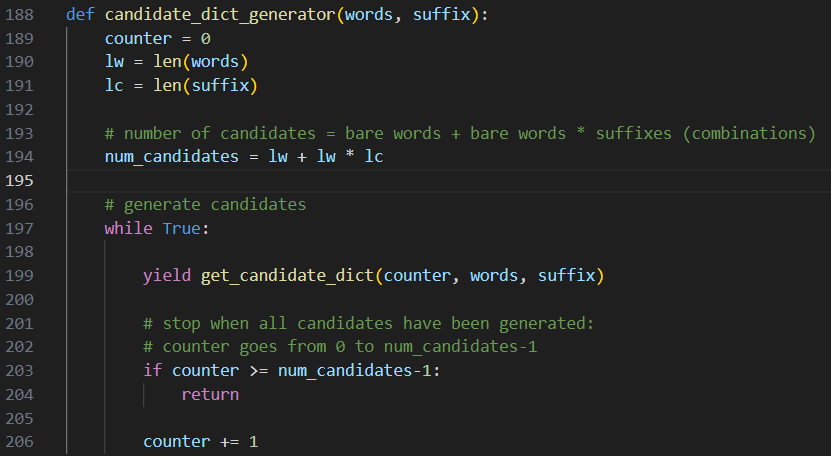
\includegraphics[width=0.8\columnwidth]{images/p1/q22.png}
				\caption{Screenshot of the modified function}
			\end{figure}
			
		\end{answer}
		
		\item (5 pts) What kind of passwords are recovered and for which users compared to Problem 0? Add a screenshot of your terminal output showing the answer. How long would it take to recover the same passwords using the bruteforce attack (Problem 0)? (Justify your answer.)
		
		\begin{answer}
			
			When comparing with the password recovered from the bruteforce attack, dictionary attack has been able to recover longer passwords for the user, James, John and David.
			
			\begin{table}[h]
				\centering
				\begin{tabular}{|l|l|}
					\hline
					\textbf{User} & \textbf{Password} \\ \hline
					James & mountain5 \\ \hline
					Robert & hat \\ \hline
					John & doughnut\# \\ \hline
					David & catcher@ \\ \hline
					Susan & pen \\ \hline
					Daniel & day2 \\ \hline
					Judy & toy \\ \hline
				\end{tabular}
				\caption{Recovered Passwords}
			\end{table}
		\begin{itemize}
			\item Time for the attack = 115.4 seconds
			\item Speed of the attack = 75130.7 hashes per second
			\item Attack success rate: 70\%
		\end{itemize}
			
				\begin{figure}[h]
				\centering
				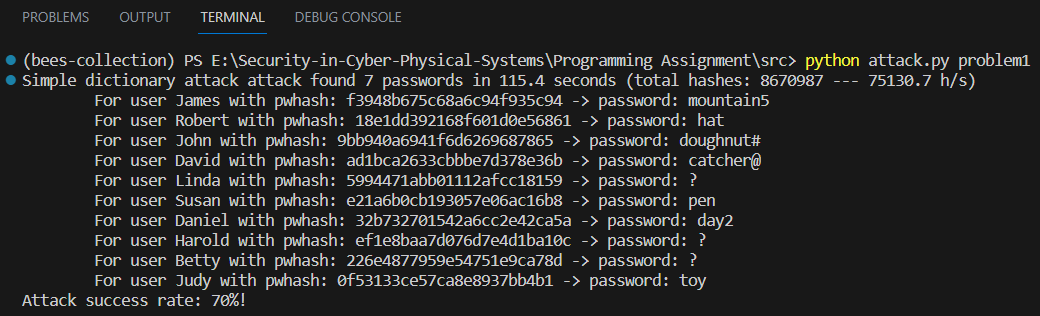
\includegraphics[width=0.7\columnwidth]{images/p1/q21.png}
				\caption{Output of the {\tt python attack.py problem1}}
			\end{figure}
			
						
			
			The longest recovered password has $l=9$ characters and they contain special characters from the list (defined in the program) in addition to the alphabet characters, therefore in total we have 26 + 36 possibilities per location in the password.\\
			
			Total number of possible passwords say $P$,
			
			\[
			P = \frac{62^{l+1}-1}{61} = \frac{62^{9+1}-1}{61} \approx 1.38 \times 10^{16}
			\]
			
			Average speed of the attack (this changes runtime-to-runtime and depending on the specifications of the machine used) therefore assume it to be $S = 60 \times 10^{3}$ hashes per second (an approximate value to the value that observed previously in problem0).\\
			
			Therefore approximate time in years say $Y$,
			
			\[
			Y = \frac{1.38 \times 10^{16}}{60 \times 10^{3}} \times \frac{1}{365 \times 24 \times 60 \times 60} \approx 7293.25 ~years 
			\]
			
			Brute force attack is not possible on this kind of passwords.
			
		\end{answer}
		
	\end{enumerate}
	
	\newpage
	\section*{Problem 2: Building a Rainbow table ({26 pts})}
	%
	
	In this problem, you will perform a Rainbow table attack against the same list of stolen password hashes (\texttt{data/simple-dbdump.json}). You will implement (part) of the password lookup rainbow table operation \texttt{lookup\_rainbow}() in \texttt{rainbow.py}. The code to build the rainbow table (\texttt{build\_rainbow}()) is provided. It will be useful to carefully read the code of \texttt{build\_rainbow}() and \texttt{test\_rainbow\_attack}() (in \texttt{attack.py}).
	
	Use the following to perform the attack:
	%
	\begin{Verbatim}
		python attack.py problem2
	\end{Verbatim}
	%
	
	%
	\begin{enumerate}
		
		\item (2 pts) How do rainbow tables differ from hash-reduce chains? Illustrate with an example.
		
		\begin{answer}
			
			%% TODO: Write your answer here.	
			Your answer here.
			
		\end{answer}
		
		\item (2 pts) Briefly explain how you determine the length of a chain and the number of chains in a rainbow table. 
		
		\begin{answer}
			
			%% TODO: Write your answer here.	
			Your answer here.
			
		\end{answer}
		
		\item (3 pts) How can you select different reduce functions to be used in different stages of the rainbow table?
		
		\begin{answer}
			
			%% TODO: Write your answer here.	
			Your answer here.
			
		\end{answer}
		
		\item (16 pts) Complete the implementation of the rainbow table attack: \texttt{lookup\_rainbow}()! Test your implementation thoroughly. Your attack should recover the same kind of passwords as for Problem~0. Add screenshots of your terminal output showing the answer and the function implementation.
		
		\begin{answer}
			
			%% TODO: Write your answer here.	
			Your answer here.
			
		\end{answer}
		
		\item (3 pts) What is a false alarm? Explain why it occurs and what we can do to minimize false alarms in rainbow tables.
		
		\begin{answer}
			
			%% TODO: Write your answer here.	
			Your answer here.
			
		\end{answer}
		
	\end{enumerate}
	
	\newpage
	\section*{Problem 3: Understanding Rainbow tables (32 pts)}
	%
	
	In this problem, you will run the Rainbow table attack on a larger database of stolen password hashes (\texttt{data/complex-dbdump.json}). Unlike for previous problems, in this step all passwords consist of 4 alphanumeric characters --- lowercase only.
	
	Use the following command to run the attack:
	%
	\begin{Verbatim}
		python attack.py problem3
	\end{Verbatim}
	%
	
	Let $n$ denote the total number of possible passwords, $m$ denote the number of chains in the rainbow table, and $k$ denote the length of each chain.
	
	\begin{enumerate}
		\item (3 pts) What is the success rate of the attack (percentage of passwords recovered)? Why is it not 100\%?
		
		\begin{answer}
			
			%% TODO: Write your answer here.	
			Your answer here.
			
		\end{answer}
		
		\item (4 pts) [Experimental] Keeping $m \cdot k$ constant, run the attack with $m = 25000$, $50000$, $100000$, $200000$, $400000$ and $k = 64, 32, 16, 8, 4$. (You can modify $m$ and $k$ in the \texttt{main}() function of \texttt{attack.py}.) 
		
		Record the success rate of the attack ($p$) and write it in the table below.
		
		\begin{answer}
			
			%% TODO: Write your answer here.	
			\begin{center}
				\begin{tabular}{l|c|c|c|c|c|}
					\hline
					$m$ & 25000 & 50000 & 100000 & 200000 & 400000 \\ \hline
					$k$ & 64 & 32    & 16      & 8      & 4      \\ \hline \hline
					$p$ &  &   &    &   &     \\ \hline
				\end{tabular}	
			\end{center}	
			
		\end{answer}
		
		\item (6 pts) Consider the case $k=1$. Observe experimentally that the success rate of the attack is lower than $\frac{m \cdot k}{n}$. Why is that?  To fix it, change the implementation of \texttt{build\_rainbow}() to ensure that each chain gets a unique startpoint. (Be careful to ensure that \texttt{build\_rainbow}() always terminates no matter the values of $n$, $m$, and $k$.)
		
		\begin{answer}
			
			%% TODO: Write your answer here.	
			Your answer here.
			
		\end{answer}
		
		\item (4 pts) [Theory] Explain the difference between hash and reduce functions and give 3 examples of possible reduce functions.
		
		\begin{answer}
			
			%% TODO: Write your answer here.	
			Your answer here.
			
		\end{answer}
		
		\item $[$Theory$]$ Assume this password-cracking algorithm is implemented on a memory-limited system. Assume that a chain can be stored using 8 bytes (4 bytes for the startpoint, 4 bytes for the endpoint). Suppose we set $m$ and $k$ such that $n = m \cdot k$. Consider the system can compute 1000 hashes per second and 1000 reduction functions per second. (Assume time taken for other instructions is negligible when compared with hashing and reduction).
		
		\begin{enumerate}
			
			\item (2 pts) What is the amount of memory required to store the rainbow table?
			
			\begin{answer}
				
				%% TODO: Write your answer here.	
				Your answer here.
				
			\end{answer}
			
			\item (3 pts) What is the expected computational complexity of a lookup?
			
			\begin{answer}
				
				%% TODO: Write your answer here.	
				Your answer here.
				
			\end{answer}
			
			\item (4 pts) Determine the optimum value for $k$ such that it uses the lowest memory space to store the rainbow table.
			
			\begin{answer}
				
				%% TODO: Write your answer here.	
				Your answer here.
				
			\end{answer}
			
		\end{enumerate}
		
		\item (6 pts) [Experimental] Keeping $m \cdot k$ constant, run the attack for $m = 25000$, $50000$, $100000$, $200000$, $400000$ and $k = 64, 32, 16, 8, 4$. Plot the time for a lookup in each case. How does this compare to your answer to Problem 3, part 5(b)?
		
		\begin{answer}
			
			%% TODO: insert your figure here (uncomment below)
			%\begin{center}
			%	\includegraphics{yourfigurefilename}
			%	\captionof{figure}{Your caption here.}     
			%\end{center}
			
			%% TODO: Write your answer here.	
			Your answer here.
			
		\end{answer}
		
	\end{enumerate}
	
	\newpage
	
	\section*{Problem 4: Bob's custom password hash (14 pts + [bonus] 10 pts)}
	%
	
	Your classmate Bob is in charge of the website of E-Club, ENTC. To implement authentication on the website, Bob (who has not taken EN4720) has decided to roll his own crypto. He has implemented a custom password hash function. Given a password $p$ of even length, $p$ is split into two parts of equal lengths $p_1$, $p_2$. The password hash is then computed as:
	\[ H_l(p_1) || H_l(p_2) || H_l^i(s || c) , \]
	where $s$ is a random salt, $c$ is a constant string, $i$ and $l$ are positive integers. Here: $H_l(x)$ denotes the first $l$ bytes of the hash of $x$. This password hash is implemented as \texttt{bobs\_custom\_pw\_hash}() in \texttt{crypto.py}.
	
	
	For this problem, you will implement your own attack against Bob's custom password hash scheme. For this you will use \texttt{data/bobX-dbdump.json} as database of password hashes.
	
	Use the following command to run your attack:
	%
	\begin{Verbatim}
		python attack.py problem4
	\end{Verbatim}
	%
	
	
	%
	\begin{enumerate}
		
		\item (2 pts) Is it a good idea to design your own crypto like Bob did in this case? Explain why or why not?
		
		\begin{answer}
			
			%% TODO: Write your answer here.	
			Your answer here.
			
		\end{answer}
		
		\item (3 pts) Give your comments on the salting mechanism used by Bob in his custom crypto. Does his method serve the purpose of salting? Explain your answer.
		
		\begin{answer}
			
			%% TODO: Write your answer here.	
			Your answer here.
			
		\end{answer}
		
		\item (3 pts)  Bob’s friend Alice says the splitting of the password into 2 equal parts and hashing them separately will make the life of an attacker difficult to launch a bruteforce attack. Do you agree with this statement? Give reasons.
		
		\begin{answer}
			
			%% TODO: Write your answer here.	
			Your answer here.
			
		\end{answer}
		
		\item (3 pts)  Is it a good idea to use the first $l$ bytes of the hashes as in Bob's crypto? Explain your answer giving reasons.
		
		\begin{answer}
			
			%% TODO: Write your answer here.	
			Your answer here.
			
		\end{answer}
		
		\item (3 pts) Suggest a suitable method to make this custom password hash scheme difficult to crack by the attackers.  
		
		\begin{answer}
			
			%% TODO: Write your answer here.	
			Your answer here.
			
		\end{answer}
		
		
		\item ([\textcolor{magenta}{bonus}] 10 pts) Implement the best attack you can think of. Place your code in the provided placeholders in \texttt{bobs\_custom\_pwhash\_attack}() (\texttt{attack.py}). You will be evaluated based on the performance of your attack on passwords of varying length. You can change the size of the targets passwords by changing the value of \texttt{pw\_length} in the \texttt{main()} function of \texttt{attack.py}.
		
		{\em Hint: the fastest attack is neither the naive bruteforce attack nor the one based on rainbow tables.}
		
		Explain how your attack works. How fast is it on passwords of length 4, 6, and 8?
		
		\begin{answer}
			
			%% TODO: Write your answer here.	
			Your answer here.
			
		\end{answer}
		
	\end{enumerate}
	
\end{document}
